Durante la creazione di una convenzione/contributo deve essere inserita una suddivisione dell'importo concordato, chiamata \textsl{ripartizione}. La ripartizione, in generale, non è totalmente libera: possono essere immessi solo alcuni valori e, sulla base di questi, ne vengono calcolati altri secondo opportuni schemi. Ad esempio, attualmente va al \textsl{Fondo Comune di Ateneo} il 2.5\% dell'ammontare totale della convenzione. \\
Il meccanismo in base al quale calcolare le quote \textquoteleft derivate\textquoteright{} a partire da quelle \textquoteleft libere\textquoteright{} può subire delle modifiche nel tempo. Per questo motivo, si è scelto di adottare il pattern \textsl{Strategy} per consentire di cambiare in un secondo momento l'algoritmo da utilizzare.\\

\subsubsection{Il pattern \textsl{Strategy}}

\begin{figure}[h]
\centering
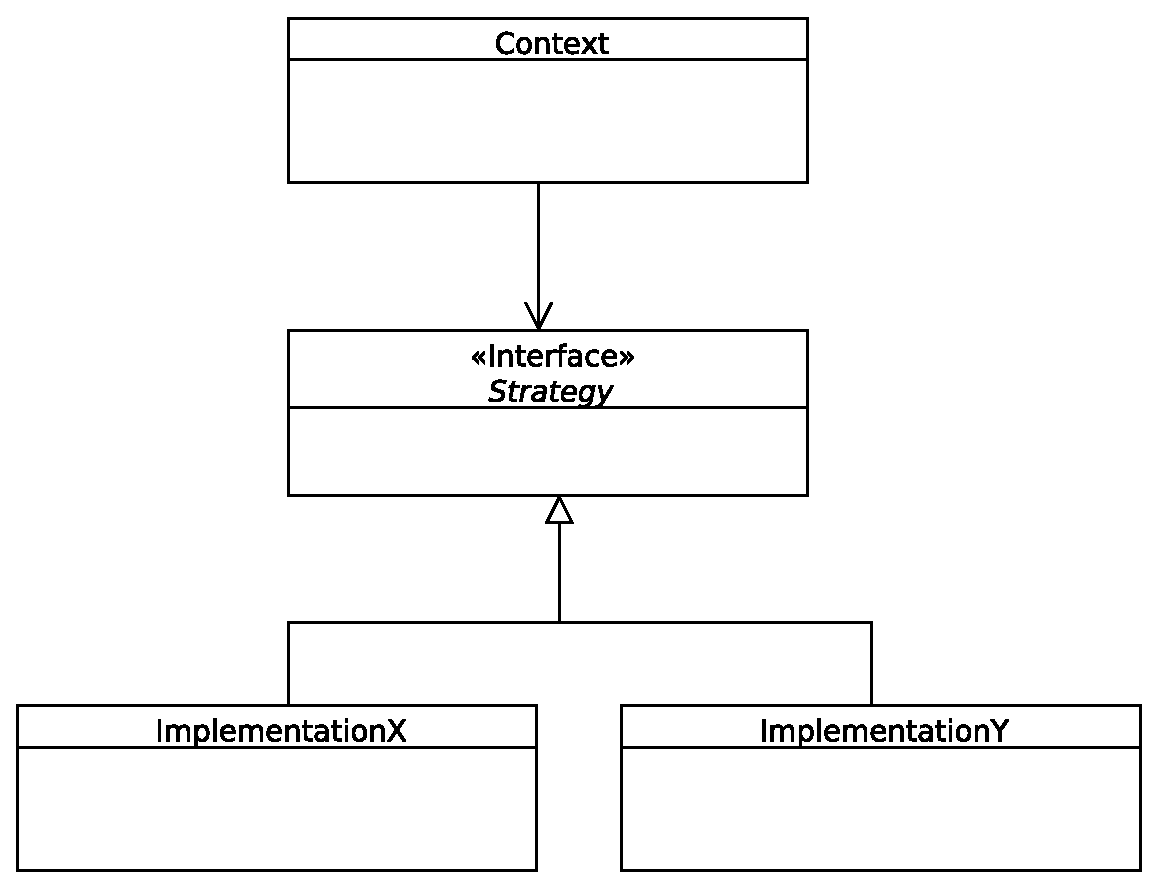
\includegraphics[width=0.6\textwidth]{strategy.eps}
\caption{Il pattern Strategy}
\label{strategy}
\end{figure}


Nel pattern Strategy, l'algoritmo è incapsulato in una classe separata rispetto al contesto in cui deve essere usato. Inoltre, tutti gli algoritmi (o meglio, tutte le classi che rappresentano un algoritmo) implementano un'interfaccia comune. L'oggetto all'interno del quale si deve adoperare un algoritmo di quel tipo avrà un riferimento all'interfaccia, rimanendo così slegata dalle classi concrete: questo rende semplice modificare in fase di manutenzione l'implementazione da utilizzare. Lo schema del pattern è raffigurato in figura \ref{strategy}; per maggiori dettagli, si consiglia \cite{gof}.\\

\subsubsection{\textsl{Filler}}

\paragraph{}
La classe che rappresenta genericamente l'algoritmo è chiamata \lstinline{ContractShareTableFiller}; per brevità, si farà di seguito riferimento ad essa con il termine \textsl{filler}. \\
Attualmente, è prevista un'unica implementazione del filler, chiamata \lstinline{StandardContractShareTableFiller} (o \textsl{filler standard}). Questa implementazione prevede tutti gli altri attributi della tabella di ripartizione vengano calcolati sulla base della quota relativa al personale. In figura \ref{filler_strategy} è mostrato il pattern Strategy applicato al caso concreto.\\
Le percentuali sulla base delle quali eseguire il calcolo sono definibili attraverso gli opportuni file di configurazione, che si trovano all'interno della sotto-cartella \path{aliquoteDipartimenti} della cartella di configurazione (path relativo alla directory di JBoss: \path{standalone/deployments/Jama.war/WEB-INF/classes/config}). \\

\begin{figure}[h]
\centering
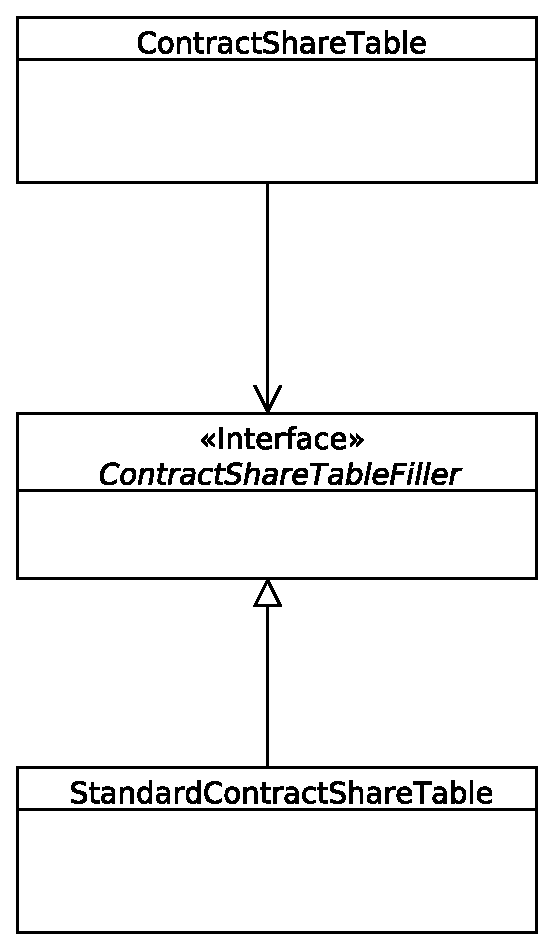
\includegraphics[width=0.25\textwidth]{filler_strategy.eps}
\caption{Il pattern Strategy applicato ai filler}
\label{filler_strategy}
\end{figure}

\paragraph{}
In realtà, in questa cartella non sono presenti file di configurazione, ma altre sotto-cartelle. Infatti, è possibile specificare aliquote diverse per ogni dipartimento, ognuno dei quali ha la propria directory, riconoscibile dall'identificativo del dipartimento stesso. Questo però ha effetti anche sul codice: non è possibile utilizzare lo stesso filler per tutti i dipartimenti. È questo il motivo per cui è stato utilizzato il pattern \textsl{Abstract factory} per incapsulare la responsabilità di istanziare il filler appropriato. Quando è necessario ottenere un filler per un dato contratto, è sufficiente chiamare il metodo \lstinline{getFiller} della factory passandogli il dipartimento del docente che lo ha stipulato. \\
Anche per la factory è necessario stabilire quale implementazione utilizzare, essendo questa legata al filler da produrre. Il meccanismo è sempre lo stesso: non si fa riferimento alla classe concreta, ma a quella di base. Se si dovesse cambiare tipo di filler, è sufficiente implementare la relativa factory ed aggiornare il resto di conseguenza. L'aggiornamento è inoltre molto più semplice nel caso della factory, perché esse non sono entità di JPA (ossia, non sono annotate \lstinline{@Entity}), ma sono bean di CDI. Questo consente di utilizzare le \textit{alternatives} (si veda il capitolo \ref{cdi} per maggiori dettagli) e quindi basta modificare il file \path{bean.xml} specificando il bean da utilizzare.\\

\paragraph{}
Le cose sono in realtà leggermente più complicate di così. Infatti, bisogna tener conto che le variazione delle quote o del metodo di calcolo stesso non devono essere retroattive. Ad esempio, se nel 2013 al Fondo Comune di Ateneo spetta il 2.5\% del totale della convenzione, mentre nel 2014 l'1\% sulla quota relativa al personale, le convenzioni stipulate nel 2013 dovranno mantenere la quota precedente (2.5\% sul totale), che siano ancora attive nel 2014 o che non lo siano. Da ciò nasce l'esigenza di aggiungere nel contratto un attributo che rappresenta il filler utilizzato e di salvare questa informazione nel database; inoltre, è necessario anche poter effettuare query sul filler stesso. Per questi motivi, nell'implementazione del pattern Strategy si è deciso di utilizzare una classe astratta invece di un'interfaccia.\\
In figura \ref{filler_complete} è mostrato lo schema completo.

\begin{figure}[h]
\centering
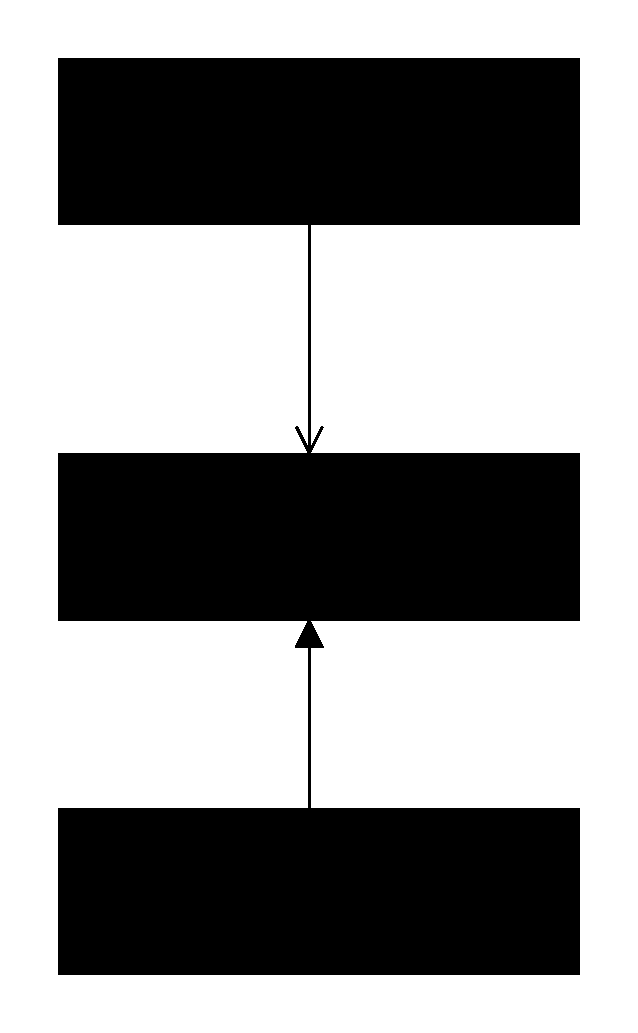
\includegraphics[width=0.6\textwidth]{filler_complete.eps}
\caption{Schema completo}
\label{filler_complete}
\end{figure}